\documentclass{article}
\usepackage{v-equation}
\usepackage{mathtools}
\geometry{
paperwidth=5in, 
paperheight=5in, 
top=10mm, 
bottom=10mm, 
left=10mm, 
right=10mm
}

\renewcommand{\d}[1]{d\!#1}
\begin{document}
\begin{center}
Rutherford and Soddy’s law
\end{center}
\vspace*{\fill}
\begin{center}

\begin{tikzpicture}
	\fill (0, 0) circle[radius=0.45];
	\foreach \a in {0, 30, ..., 330}{
		\tzsnake[->](\a:0.7cm)(\a:1.8cm)
		\fill (\a:2cm) circle(3pt);
	}
\end{tikzpicture}
\end{center}
\begin{align*}
-\dfrac{\d{N}}{\d{t}} &\propto N \\
-\dfrac{\d{N}}{\d{t}} &= \lambda N\\
\int_{N_0}^{N} \dfrac{\d{N}}{N} &= -\lambda \int_0^t \d{t}\\
\ln\left( \dfrac{N}{N_0} \right) &= -\lambda t \\
\Aboxed{N &= N_0e^{-\lambda t}}
\end{align*}
\vspace*{\fill}

\pagebreak
\begin{center}
\begin{tikzpicture}
[yscale=0.8]
	\def\Fn{3*exp(-0.5*\x)}
	\tzaxes(-0.5, -0.5)(7, 4){$t$}{$N$}
	\tzfn\Fn[0:5]
	\tzfn[dashed]\Fn[5:6.5]
	\tzticksy(-2pt:2pt){3/$N_0$}
\end{tikzpicture}
\end{center}
\vspace*{\fill}

\begin{align*}
N &- \texttt{number of nuclei at time $t$}\\
N_0 &- \texttt{number of nuclei at time $t=0$}\\
\lambda &- \texttt{decay constant}\\
t &- \texttt{time}\\
\end{align*}

\vspace*{\fill}

\begin{center}
	\fbox{\qrcode[height=2cm]{https://drive.google.com/drive/folders/1Hj9NFANyb9FOssB9wrDKJLsjuZAJdss_?usp=share_link}}
\end{center}
\end{document}
